\begin{frame}
\frametitle{Définitions Fondamentales des Graphes}

\begin{tcolorbox}[colback=orange!10,colframe=orange!100!black,
    title=Un Chemin]
    Un \textbf{Chemin} est une séquence de sommets connectés par des arêtes.
\end{tcolorbox}

\begin{figure}[H]
    \centering
    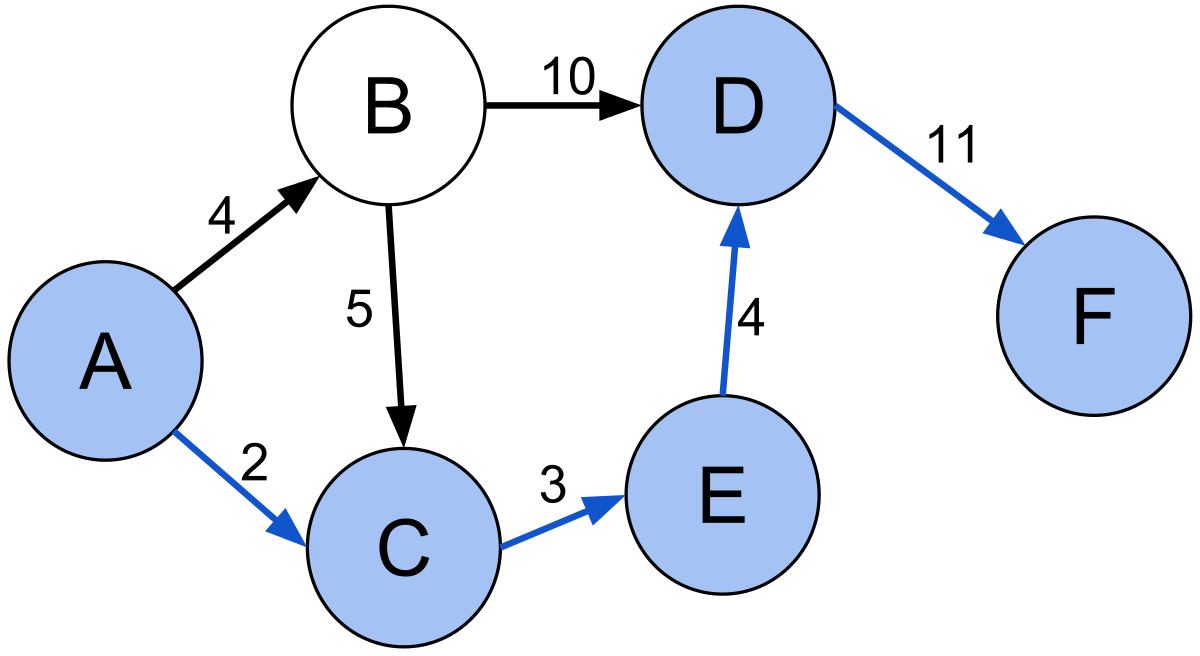
\includegraphics[width=0.5 \textwidth]{Figures/chemin.png}
    \caption{Un Chemin}
    \label{fig:Un Chemin}
\end{figure}

\end{frame}